\section{映射后的密度}
\label{sec:push-mapped-densities}

推前积分恒等式把目标空间上的积分送回原空间。但在目标空间上直接计算时，我们往往希望把推前测度写成一个熟悉的参考测度的加权形式，就像在实轴上用概率密度代替分布本身。

设在目标空间$Y$上选定参考测度$\lambda$，并假设推前测度有密度
\[
h=\frac{\mathrm d(T_\#\mu)}{\mathrm d\lambda}.
\]
对非负可测$g$，连续使用推前积分恒等式与第~\ref{chap:measure-densities}章的换测度公式，得到两步改写
\begin{equation}
\int_Xg\circ T\,\mathrm d\mu=\int_Yg\,\mathrm d(T_\#\mu)=\int_Ygh\,\mathrm d\lambda .
\label{eq:push-two-step}
\end{equation}

第一步沿映射转移测度并复合被积函数，第二步留在$Y$上，只把累计权重换成$h$。两步依据不同的定理，条件也不同：第一步对任何可测映射成立，第二步要求密度存在。

\paragraph{密度未必存在}
密度存在的必要条件是$T_\#\mu\ll\lambda$，即对每个$\lambda$零测集$N\subset Y$，都有
\[
\mu\bigl(T^{-1}(N)\bigr)=0 .
\]
也就是说，映射不能把正的质量压进目标空间的零测集。

常值映射给出最简单的反例。令$X=[0,1]$，$\mu=\lambda|_{[0,1]}$，$T(x)=c$。当$c\in B$时$T^{-1}(B)=[0,1]$，否则$T^{-1}(B)=\varnothing$，所以
\[
T_\#\mu=\delta_c .
\]
单点$\{c\}$是Lebesgue零测集，却承载全部质量，$T_\#\mu$与$\lambda$相互奇异，没有Lebesgue密度。映射把一段区间压成一点，原像$T^{-1}(\{c\})$有正长度，这就是失败的原因。

所以计算映射后的密度，要先确认映射不把正质量压进零测集。下面三个小节分别处理三种常见结构：光滑可逆映射、分成有限个可逆光滑分支的映射，以及坐标投影。

\subsection{光滑坐标换元}
\label{sec:push-smooth-change}

设$U,V\subset\mathbb R^d$是开集。若$T:U\to V$是双射，$T$与$T^{-1}$都连续可微，就称$T$为$C^1$\term{微分同胚}（diffeomorphism）。对$T^{-1}\circ T=\mathrm{id}$求导，得
\[
DT^{-1}\bigl(T(\bm x)\bigr)\,DT(\bm x)=\bm I .
\]

取行列式可知\term{Jacobian行列式}（Jacobian determinant）$\det DT(\bm x)$处处不为零，并且
\begin{equation}
\bigl\lvert\det DT^{-1}(\bm y)\bigr\rvert=\frac{1}{\bigl\lvert\det DT\bigl(T^{-1}(\bm y)\bigr)\bigr\rvert},\qquad\bm y\in V .
\label{eq:push-inverse-jacobian}
\end{equation}
本小节记$S=T^{-1}:V\to U$，它也是$C^1$微分同胚。所有函数与集合都取Borel可测的版本。

\paragraph{Lebesgue测度的推前}
先以$\lambda_d|_U$为原测度，问它推前到$V$上是什么。由定义，小盒子$Q\subset V$得到的质量是它的原像$S(Q)$的体积。$S$在小盒子上近似于线性映射$DS(\bm y)$，线性映射把体积乘以行列式的绝对值，所以
\[
(T_\#\lambda_d)(Q)=\lambda_d\bigl(S(Q)\bigr)\approx\bigl\lvert\det DS(\bm y)\bigr\rvert\,\lambda_d(Q).
\]
这说明推前测度的密度应当是逆映射的Jacobian因子。

用极坐标算一个具体的小盒子。取$S(r,\theta)=(r\cos\theta,r\sin\theta)$，$T$是它的逆，Jacobian行列式为
\[
\det DS(r,\theta)=r .
\]
取$Q=[1,1.2]\times[0.3,0.8]$，它的面积是$0.2\times0.5=0.1$。它的原像$S(Q)$是一块环形扇区，面积是
\[
\lambda_2\bigl(S(Q)\bigr)=\int_{0.3}^{0.8}\int_1^{1.2}r\,\mathrm dr\,\mathrm d\theta=0.5\times\frac{1.2^2-1^2}{2}=0.11 .
\]

两个面积之比是$0.11/0.1=1.1$，恰好是$Q$中心$r=1.1$处的$\lvert\det DS\rvert$。图~\ref{fig:push-local-volume}画出了这个小盒子和它的原像。绿色虚线是线性化$DS$给出的平行四边形，面积也是$1.1\times0.1=0.11$；它与真实的环形扇区只差一些边角，盒子越小差得越少。

\begin{BookInlineFigure}
  \centering
  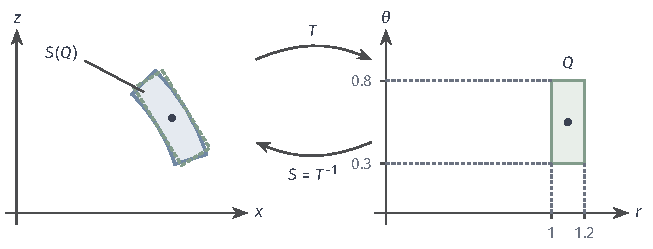
\includegraphics[width=110.539mm]{figures/04-spaces-measures-and-geometry/02-measure/tikz/push-local-volume/figure.pdf}
  \caption{小盒子的原像决定局部密度。右图是极坐标平面上的盒子$Q=[1,1.2]\times[0.3,0.8]$，左图蓝色区域是它在$(x,z)$平面的原像$S(Q)$，绿色虚线是中心处线性化$DS$给出的平行四边形，黑点是中心。两张图用相同的比例尺，面积分别为$0.1$与$0.11$，比值$1.1$等于$\lvert\det DS\rvert$在中心的值。}
  \label{fig:push-local-volume}
\end{BookInlineFigure}

把这个局部比例严格化，需要卷二的经典换元公式。设$E\subset V$是紧Jordan区域，$S(E)$也是Jordan区域，$f$在$S(E)$上连续，则
\begin{equation}
\int_{S(E)}f(\bm x)\,\mathrm d\bm x=\int_Ef\bigl(S(\bm y)\bigr)\,\lvert\det DS(\bm y)\rvert\,\mathrm d\bm y .
\label{eq:push-classical-change}
\end{equation}
公式的陈述和证明思路见\BookChapterRef{chap:region-integrals}{卷二第24章“区域积分”}。证明需要对细分作一致的误差控制，篇幅较长，读者可查阅实分析教材。我们只用它在闭盒子上、$f\equiv1$时的情形，再用测度延拓的唯一性推广到一切Borel集。

\begin{theorem}[微分同胚下Lebesgue测度的推前]
\label{thm:push-lebesgue-diffeo}
设$T:U\to V$是$C^1$微分同胚。则对每个Borel集$B\subset V$，
\begin{equation}
(T_\#\lambda_d)(B)=\lambda_d\bigl(T^{-1}(B)\bigr)=\int_B\bigl\lvert\det DT^{-1}(\bm y)\bigr\rvert\,\mathrm d\bm y ,
\label{eq:push-lebesgue-diffeo}
\end{equation}
即$T_\#(\lambda_d|_U)$相对于$\lambda_d|_V$的密度是$\lvert\det DT^{-1}\rvert$。
\end{theorem}

\begin{proof}
令$\nu(B)=\int_B\lvert\det DS\rvert\,\mathrm d\bm y$，它是$V$的Borel集上的测度。证明分两步：先在闭盒子上比较$T_\#\lambda_d$与$\nu$，再推广到全部Borel集。

设$Q\subset V$是闭盒子，允许退化。$S$是同胚，所以$S(Q)$是紧集，边界是$S(\partial Q)$。$S$在凸紧集$Q$上连续可微，由中值不等式在$Q$上Lipschitz，因而把$Q$中容量为零的集合映成容量为零的集合。$\partial Q$的容量为零，所以$S(\partial Q)$的容量为零，$S(Q)$是紧Jordan区域。

对$E=Q$、$f\equiv1$用式~\eqref{eq:push-classical-change}。Jordan区域上连续函数的Riemann积分等于Lebesgue积分，于是
\[
(T_\#\lambda_d)(Q)=\lambda_d\bigl(S(Q)\bigr)=\int_Q\lvert\det DS(\bm y)\rvert\,\mathrm d\bm y=\nu(Q).
\]

含于$V$的闭盒子连同空集对有限交封闭，构成$\pi$系统。$V$的每个开子集都是可数个含于其中的有理端点闭盒子之并，所以这些盒子生成$V$上的Borel $\sigma$代数，并有可数个覆盖$V$。两个测度在每个闭盒子上都有限，因为$S(Q)$紧、$\lvert\det DS\rvert$在$Q$上有界。由第~\ref{chap:measure}章的延拓唯一性，$T_\#\lambda_d=\nu$在$V$的全部Borel集上成立。
\end{proof}

定理说明，推前测度的密度在新坐标$\bm y$处取值，因子是逆映射的Jacobian。由式~\eqref{eq:push-inverse-jacobian}，它也可以写成$1/\lvert\det DT(S(\bm y))\rvert$：$T$在原像附近把体积拉伸的地方，同样多的质量摊到更大的范围，密度就变小。

\paragraph{原测度有密度的情形}
现在设$U$上的测度$\mu$相对于$\lambda_d$有密度$p$。把推前积分恒等式、换测度公式与上一个定理接起来，就得到推前测度的密度。

\begin{theorem}[微分同胚下的推前密度]
\label{thm:push-density-diffeo}
设$T:U\to V$是$C^1$微分同胚，$U$上的测度$\mu$相对于$\lambda_d$有密度$p$。则$T_\#\mu$相对于$V$上的$\lambda_d$有密度
\begin{equation}
q(\bm y)=p\bigl(T^{-1}(\bm y)\bigr)\,\bigl\lvert\det DT^{-1}(\bm y)\bigr\rvert ,\qquad\bm y\in V .
\label{eq:push-density-diffeo}
\end{equation}
\end{theorem}

\begin{proof}
设$B\subset V$是Borel集。由推前测度和密度的定义，
\[
(T_\#\mu)(B)=\mu\bigl(T^{-1}(B)\bigr)=\int_U\mathbf 1_B\bigl(T(\bm x)\bigr)\,p(\bm x)\,\mathrm d\bm x .
\]

因为$\bm x=S(T(\bm x))$，被积函数可以写成$\psi\circ T$，其中
\[
\psi(\bm y)=\mathbf 1_B(\bm y)\,p\bigl(S(\bm y)\bigr)
\]
是$V$上的非负Borel函数。对$\lambda_d|_U$与$T$用推前积分恒等式，再用定理~\ref{thm:push-lebesgue-diffeo}的密度与换测度公式，得到
\[
\begin{aligned}
\int_U\psi\circ T\,\mathrm d\lambda_d&=\int_V\psi\,\mathrm d(T_\#\lambda_d)\\
&=\int_V\psi(\bm y)\,\lvert\det DS(\bm y)\rvert\,\mathrm d\bm y\\
&=\int_Bp\bigl(S(\bm y)\bigr)\,\lvert\det DS(\bm y)\rvert\,\mathrm d\bm y .
\end{aligned}
\]
这正是$(T_\#\mu)(B)=\int_Bq\,\mathrm d\lambda_d$。
\end{proof}

\paragraph{与通常换元公式对照}
通常的积分换元公式中出现的是正向的Jacobian，这与定理~\ref{thm:push-density-diffeo}的因子方向相反。它也可以由定理~\ref{thm:push-lebesgue-diffeo}得到：把定理用于微分同胚$S:V\to U$，得到$S_\#\lambda_d$的密度是$\lvert\det DS^{-1}\rvert=\lvert\det DT\rvert$。

对非负Borel函数$g$，把$g$写成$(g\circ T)\circ S$，用推前积分恒等式，再用这个密度，得到
\begin{equation}
\begin{aligned}
\int_Vg\,\mathrm d\lambda_d&=\int_V(g\circ T)\circ S\,\mathrm d\lambda_d\\
&=\int_Ug\circ T\,\mathrm d(S_\#\lambda_d)\\
&=\int_Ug\bigl(T(\bm x)\bigr)\,\lvert\det DT(\bm x)\rvert\,\mathrm d\bm x .
\end{aligned}
\label{eq:push-jacobian-change}
\end{equation}

两个公式回答不同的问题。式~\eqref{eq:push-density-diffeo}问的是“新坐标$\bm y$处每单位体积有多少质量”，所以因子在新坐标上取值，是逆映射的Jacobian。式~\eqref{eq:push-jacobian-change}把新坐标上的体积元改写到原坐标上，所以因子在原坐标上取值，是正向映射的Jacobian。

用第~\ref{sec:push-mass-transfer}小节的伸缩$T(x)=2x$核对方向。这时$T^{-1}(y)=y/2$，导数的绝对值是$\tfrac12$，由定理~\ref{thm:push-lebesgue-diffeo}，
\[
T_\#\lambda=\tfrac12\lambda ,
\]
与按原像直接计算的结果一致：拉长一倍，密度减半。

而式~\eqref{eq:push-jacobian-change}给出
\[
\int g(y)\,\mathrm dy=\int g(2x)\cdot2\,\mathrm dx ,
\]
因子是正向导数$T'=2$：原坐标的一小段$\mathrm dx$，在新坐标中长$2\,\mathrm dx$。把两个因子混用，密度会算成实际值的四倍或四分之一。

\begin{example}[指数分布与仿射变换]
\label{ex:push-exponential}
取$(0,1)$上的均匀概率测度，密度$p=1$，经$T(x)=-\ln x$映到$(0,+\infty)$。逆映射与导数分别是
\[
T^{-1}(y)=\mathrm e^{-y},\qquad\bigl\lvert(T^{-1})'(y)\bigr\rvert=\mathrm e^{-y}.
\]

由式~\eqref{eq:push-density-diffeo}，输出密度是
\[
q(y)=\mathrm e^{-y},\qquad y>0 ,
\]
这是指数分布，总质量$\int_0^\infty\mathrm e^{-y}\,\mathrm dy=1$。

核对一个集合。$(1,2]$的原像是$[\mathrm e^{-2},\mathrm e^{-1})$，于是
\[
(T_\#\mu)\bigl((1,2]\bigr)=\mathrm e^{-1}-\mathrm e^{-2}=\int_1^2\mathrm e^{-y}\,\mathrm dy .
\]

再看仿射变换$T(\bm x)=\bm A\bm x+\bm b$，其中$\bm A$可逆。逆映射是$\bm A^{-1}(\bm y-\bm b)$，Jacobian因子是常数$1/\lvert\det\bm A\rvert$，所以
\[
q(\bm y)=\frac{p\bigl(\bm A^{-1}(\bm y-\bm b)\bigr)}{\lvert\det\bm A\rvert}.
\]
\end{example}

图~\ref{fig:push-exponential-bins}把指数分布例子中的密度“算”了出来。把$(0,1)$分成长度$0.2$的小段，每段质量都是$0.2$。靠近$x=1$的小段$(0.8,1)$映到长度约$0.223$的区间，平均高度约$0.2/0.223\approx0.90$；$(0.2,0.4]$映到长度约$0.693$的区间，平均高度约$0.29$。$T$拉得越长的地方，矩形越矮，这些矩形的高度沿着$\mathrm e^{-y}$下降。

\begin{BookInlineFigure}
  \centering
  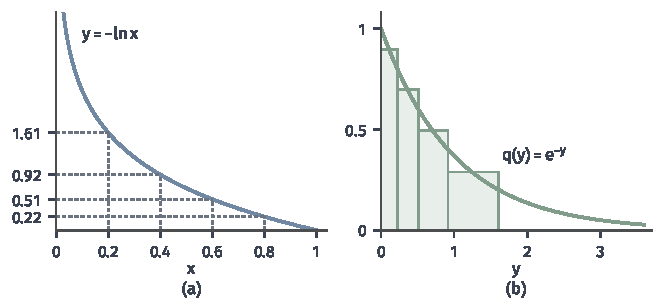
\includegraphics[width=112mm]{figures/04-spaces-measures-and-geometry/02-measure/matplotlib/push-exponential-bins/figure.pdf}
  \caption{由等质量分割看推前密度。(a)映射$y=-\ln x$与$x=0.2,0.4,0.6,0.8$对应的$y$值。(b)绿色矩形的底是长度$0.2$的输入小段映成的区间，面积都是$0.2$，所以高度等于$0.2$除以区间长度；曲线是极限密度$q(y)=\mathrm e^{-y}$。最左的输入小段$(0,0.2]$映到$[1.61,+\infty)$，质量$0.2$落在右侧的尾部，图中未画矩形。}
  \label{fig:push-exponential-bins}
\end{BookInlineFigure}

\subsection{多分支映射}
\label{sec:push-branches}

许多映射不是整体可逆的。$T(x)=x^2$把$x$与$-x$送到同一点，但在$(0,1)$与$(-1,0)$上分别是微分同胚。这类映射的处理办法是把定义域分成几块，在每块上用上一小节的公式，再把落到同一目标点的贡献加起来。

\begin{theorem}[分支映射的推前密度]
\label{thm:push-branch-density}
设$U\subset\mathbb R^d$是开集，$U_1,\ldots,U_m\subset U$是两两不交的开集，例外集$E=U\setminus\bigcup_kU_k$是Lebesgue零测集。设$T:U\to\mathbb R^d$可测，并且每个限制$T_k=T|_{U_k}$是$U_k$到开集$V_k=T(U_k)$的$C^1$微分同胚，$S_k=T_k^{-1}$。若$U$上的测度$\mu$相对于$\lambda_d$有密度$p$，则$T_\#\mu$相对于$\lambda_d$有密度
\begin{equation}
q(\bm y)=\sum_{k=1}^m\mathbf 1_{V_k}(\bm y)\,p\bigl(S_k(\bm y)\bigr)\,\bigl\lvert\det DS_k(\bm y)\bigr\rvert .
\label{eq:push-branch-density}
\end{equation}
\end{theorem}

\begin{proof}
对Borel集$B\subset\mathbb R^d$，把原像按分支拆开，
\[
T^{-1}(B)=\bigl(T^{-1}(B)\cap E\bigr)\cup\bigcup_{k=1}^m\bigl(T^{-1}(B)\cap U_k\bigr),
\]
各部分两两不交。$\mu\ll\lambda_d$，所以$\mu(E)=0$，第一部分不贡献质量。

在第$k$块上，$T^{-1}(B)\cap U_k=T_k^{-1}(B\cap V_k)$。把定理~\ref{thm:push-density-diffeo}用于$T_k$与$U_k$上的测度$\mu|_{U_k}$，其密度是$p$在$U_k$上的限制，得到
\[
\mu\bigl(T_k^{-1}(B\cap V_k)\bigr)=\int_{B\cap V_k}p\bigl(S_k(\bm y)\bigr)\,\lvert\det DS_k(\bm y)\rvert\,\mathrm d\bm y .
\]

对$k$求和，有限个非负积分之和等于和的积分，于是$(T_\#\mu)(B)=\int_Bq\,\mathrm d\lambda_d$。
\end{proof}

定理的三个条件各管一件事。分支两两不交，保证每个原像点只计算一次。例外集$E$是零测集，保证没有遗漏质量；若$T$在一段正长度的区间上取常值，这段不能纳入任何分支，那里可能产生原子，必须另行计算。

各分支的像$V_k$可以重叠。重叠处的点有多个原像，每个原像所在的分支都贡献一项，所以要求和；只取一个逆分支会漏掉其余原像处的质量。可数个分支的情形也成立，此时交换求和与积分的依据是单调收敛定理。

\begin{example}[平方映射]
\label{ex:push-square}
取$[-1,1]$上的均匀概率测度，密度$p=\tfrac12$，$T(x)=x^2$。端点的质量为零，取$U=(-1,1)$。两个分支是$U_1=(0,1)$与$U_2=(-1,0)$，例外集$E=\{0\}$是零测集；两支的像都是$(0,1)$，逆映射分别是
\[
S_1(y)=\sqrt y,\qquad S_2(y)=-\sqrt y ,
\]
导数的绝对值都是$1/(2\sqrt y)$。由式~\eqref{eq:push-branch-density}，在$0<y<1$上
\[
q(y)=\frac12\cdot\frac{1}{2\sqrt y}+\frac12\cdot\frac{1}{2\sqrt y}=\frac{1}{2\sqrt y},
\]
在$(0,1)$外$q=0$。总质量是
\[
\int_0^1\frac{\mathrm dy}{2\sqrt y}=\bigl[\sqrt y\bigr]_0^1=1 .
\]

核对一个集合。取$B=[0.36,0.49]$，原像是$[-0.7,-0.6]\cup[0.6,0.7]$，总长度$0.2$，输入质量是
\[
0.2\times\tfrac12=0.1 .
\]
用输出密度计算，
\[
\int_{0.36}^{0.49}\frac{\mathrm dy}{2\sqrt y}=0.7-0.6=0.1 .
\]
若只取正分支，得到的$1/(4\sqrt y)$总积分只有$\tfrac12$，漏掉了另一半质量。
\end{example}

图~\ref{fig:push-square}左侧显示了例子中的计算：黄色带是输出区间$B$，它在曲线上碰到两个分支，往下落到两段蓝色的输入区间，各贡献质量$0.05$。右侧是相加后的密度，虚线是只取一个分支时的结果。

\begin{BookInlineFigure}
  \centering
  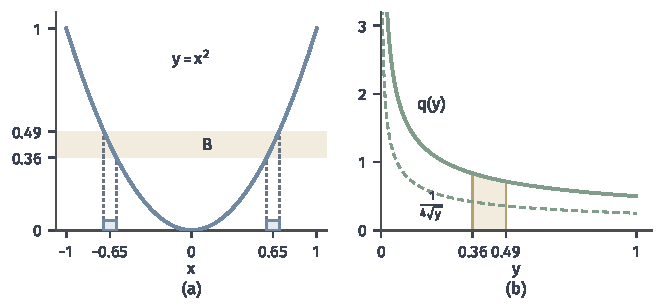
\includegraphics[width=112mm]{figures/04-spaces-measures-and-geometry/02-measure/matplotlib/push-square/figure.pdf}
  \caption{平方映射的推前密度。(a)映射$y=x^2$；输出区间$B=[0.36,0.49]$（黄色带）有两个原像$[-0.7,-0.6]$与$[0.6,0.7]$（蓝色）。(b)实线是两支相加的密度$q(y)=1/(2\sqrt y)$，虚线是只取一个分支的$1/(4\sqrt y)$；$B$上实线下的面积是$0.1$，与输入质量一致。纵轴在$3.2$处截断，$y\to0$时$q$无界但可积。}
  \label{fig:push-square}
\end{BookInlineFigure}

输出密度在$y\to0$时无界，但仍可积。原点的原像只有单点$\{0\}$，输入质量为$0$，所以输出没有点质量。若输入在$0$处有点质量，例如换成$\tfrac12\delta_0+\tfrac14\lambda|_{[-1,1]}$，原测度就不再相对于$\lambda$绝对连续，定理不适用；推前后在$0$处出现点质量$\tfrac12$，这部分不能用相对于长度的密度表示。

\subsection{坐标投影}
\label{sec:push-projection-density}

坐标投影也是多对一映射，但与上一小节不同：落到同一点$x_1$的原像不是有限个点，而是整条\term{纤维}（fiber）$\{x_1\}\times X_2$，其上每一点的质量通常为零。有限分支求和在这里无从谈起，应当沿纤维积分。为此需要原测度相对于乘积参考测度有密度。

\begin{theorem}[边缘密度]
\label{thm:push-marginal-density}
设$(X_1,\mathcal A_1,\mu_1)$与$(X_2,\mathcal A_2,\mu_2)$是$\sigma$有限测度空间，$X_1\times X_2$上的测度$\mu$相对于乘积测度$\mu_1\otimes\mu_2$有密度$p$，$\pi(x_1,x_2)=x_1$。则$\pi_\#\mu$相对于$\mu_1$有密度
\begin{equation}
p_1(x_1)=\int_{X_2}p(x_1,x_2)\,\mu_2(\mathrm dx_2).
\label{eq:push-marginal-density}
\end{equation}
\end{theorem}

\begin{proof}
对$B\in\mathcal A_1$，原像是$\pi^{-1}(B)=B\times X_2$。由密度的定义，再对非负函数用Tonelli定理，
\[
\begin{aligned}
(\pi_\#\mu)(B)&=\mu(B\times X_2)\\
&=\int_{X_1\times X_2}\mathbf 1_B(x_1)\,p(x_1,x_2)\,\mathrm d(\mu_1\otimes\mu_2)\\
&=\int_B\Bigl(\int_{X_2}p(x_1,x_2)\,\mu_2(\mathrm dx_2)\Bigr)\mu_1(\mathrm dx_1).
\end{aligned}
\]
Tonelli定理同时保证内层积分$p_1$是$x_1$的可测函数。于是$(\pi_\#\mu)(B)=\int_Bp_1\,\mathrm d\mu_1$。
\end{proof}

$p_1$取值于$[0,+\infty]$。若$\mu$有限，取$B=X_1$得
\[
\int_{X_1}p_1\,\mathrm d\mu_1=\mu(X_1\times X_2)<+\infty ,
\]
所以$p_1$在$\mu_1$几乎处处有限。

被积函数非负，用Tonelli定理就够了；若要对有符号的$g(x_1)$计算$\int g\,\mathrm d(\pi_\#\mu)$，则要先确认$\int\lvert g\rvert p_1\,\mathrm d\mu_1<+\infty$，这时Fubini定理保证换序。

参考测度取计数测度时，式~\eqref{eq:push-marginal-density}中的积分变成对第二个坐标求和，就是离散联合分布求边缘的公式，也就是图~\ref{fig:push-projection}中逐行逐列的合计。

\begin{example}[正方形上的线性密度]
\label{ex:push-square-marginal}
在$[0,1]^2$上取$\mu$相对于$\lambda_2$的密度$p(x,z)=x+z$。总质量是
\[
\int_0^1\!\!\int_0^1(x+z)\,\mathrm dz\,\mathrm dx=\int_0^1\bigl(x+\tfrac12\bigr)\,\mathrm dx=1 .
\]

第一坐标的边缘密度由式~\eqref{eq:push-marginal-density}算出：
\[
p_1(x)=\int_0^1(x+z)\,\mathrm dz=x+\tfrac12,\qquad0\leq x\leq1 .
\]

核对一个集合。用边缘密度计算，
\[
(\pi_\#\mu)\bigl([0,\tfrac12]\bigr)=\int_0^{1/2}\bigl(x+\tfrac12\bigr)\,\mathrm dx=\tfrac18+\tfrac14=\tfrac38 .
\]
直接用原测度计算，
\[
\mu\bigl([0,\tfrac12]\times[0,1]\bigr)=\int_0^{1/2}\!\!\int_0^1(x+z)\,\mathrm dz\,\mathrm dx=\tfrac38 ,
\]
两者相同。
\end{example}

图~\ref{fig:push-marginal-fiber}把例子中的一条纤维单独取出来。在$x=0.3$处，纤维是竖直的线段，密度沿纤维是$0.3+z$，积分得到$0.3+\tfrac12=0.8$，这就是$p_1(0.3)$。对每个$x$做一次这样的积分，$p_1$的整条曲线就出来了。

\begin{BookInlineFigure}
  \centering
  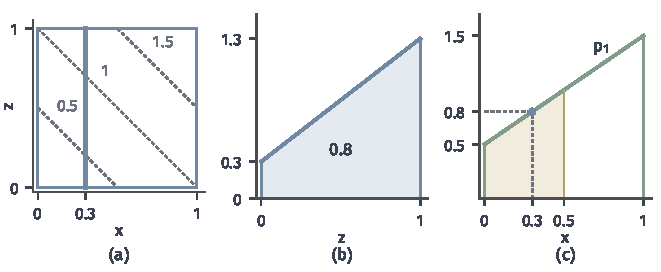
\includegraphics[width=112mm]{figures/04-spaces-measures-and-geometry/02-measure/matplotlib/push-marginal-fiber/figure.pdf}
  \caption{沿纤维积分得到边缘密度。(a)单位正方形上$p(x,z)=x+z$的等值线（虚线，数字是$p$的值），粗线是$x=0.3$处的纤维。(b)沿这条纤维的密度$0.3+z$，阴影面积$0.8$。(c)边缘密度$p_1(x)=x+\tfrac12$，蓝点是(b)算出的值，黄色面积是$[0,\tfrac12]$上的质量$\tfrac38$。}
  \label{fig:push-marginal-fiber}
\end{BookInlineFigure}

\paragraph{与分支求和的区别}
投影与分支映射都是多对一的，但累计方式不同。分支映射的每个目标点只有有限个原像，每个原像附近映射是局部微分同胚，贡献由Jacobian因子换算后相加。投影的原像是整条纤维，纤维上单点没有质量，贡献必须用纤维上的参考测度$\mu_2$积分。表~\ref{tab:push-mechanisms}汇总了本节的三种机制。

\begin{BookInlineTable}
  \centering
  \begin{tabular}{@{}llll@{}}
    \toprule
    & 微分同胚 & 多分支映射 & 坐标投影\\
    \midrule
    目标点的原像 & 一个点 & 有限个点 & 一条纤维\\
    参考测度 & Lebesgue测度 & Lebesgue测度 & 乘积测度\\
    密度的来源 & 逆映射Jacobian & 各分支相加 & 沿纤维积分\\
    依据 & 经典换元公式 & 逐分支换元 & Tonelli定理\\
    \bottomrule
  \end{tabular}
  \caption{三种计算推前密度的机制。}
  \label{tab:push-mechanisms}
\end{BookInlineTable}

累次积分的依据是乘积结构：$\mu$的参考测度是乘积测度，纤维恰好是坐标截面。一般的非线性降维没有现成的乘积结构，必须另行核对沿纤维积分的条件，以及纤维上用什么参考测度。一种可行的做法是先用微分同胚把纤维拉直成坐标截面，再投影。

以单位圆盘$D$上的均匀概率测度为例，密度是$1/\pi$，映射$R(x,z)=\sqrt{x^2+z^2}$把点送到它到原点的距离，纤维是同心圆周。为把圆周拉直，先去掉零测的射线$\{(x,0):x\geq0\}$，此后极坐标
\[
\Phi(r,\theta)=(r\cos\theta,r\sin\theta)
\]
是$G=(0,1)\times(0,2\pi)$到圆盘剩余部分的微分同胚，Jacobian行列式是$r$。

令$T=\Phi^{-1}$，由式~\eqref{eq:push-density-diffeo}，$T_\#\mu$相对于$G$上面积的密度是
\[
q(r,\theta)=\frac1\pi\cdot r=\frac r\pi .
\]
$R$就是$T$与第一坐标投影$\pi_1$的复合，由复合规则~\eqref{eq:push-composition}和定理~\ref{thm:push-marginal-density}，半径的密度是
\[
p_R(r)=\int_0^{2\pi}\frac r\pi\,\mathrm d\theta=2r,\qquad0<r<1 .
\]

核对一个集合：半径不超过$s$的质量是面积比$s^2$，而$\int_0^s2r\,\mathrm dr=s^2$。图~\ref{fig:push-polar-fibers}中的黄色环带取$0.5<r\leq0.6$，三幅图里的质量都是$0.6^2-0.5^2=0.11$。

\begin{BookInlineFigure}
  \centering
  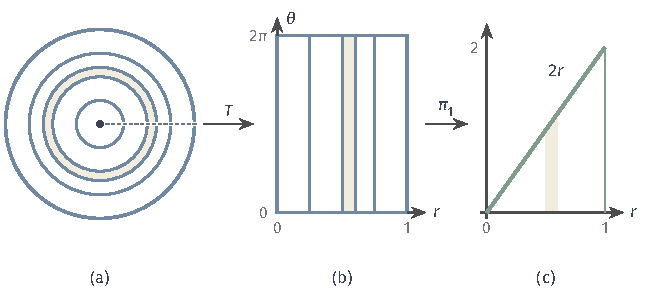
\includegraphics[width=109.813mm]{figures/04-spaces-measures-and-geometry/02-measure/tikz/push-polar-fibers/figure.pdf}
  \caption{先把纤维拉直再投影。(a)单位圆盘上$R(x,z)=\sqrt{x^2+z^2}$的几条纤维（同心圆周），虚线是去掉的射线。(b)极坐标平面上，同一批纤维变成竖直线段。(c)对$\theta$积分后得到半径的密度$2r$。黄色部分是$0.5<r\leq0.6$的同一批点，质量都是$0.11$。}
  \label{fig:push-polar-fibers}
\end{BookInlineFigure}

这个例子说明纤维上的参考测度不能想当然。直接对$\theta$积分平面密度$1/\pi$，得到常数$2$，总质量变成$2$，这是漏掉了Jacobian因子$r$。沿圆周用弧长积分$1/\pi$，得到$2\pi r/\pi=2r$，结果正确；但这个正确是有条件的。

换一个输出函数$t=x^2+z^2$，纤维还是同样的圆周。由半径的密度$2r$和映射$r\mapsto r^2$，用式~\eqref{eq:push-density-diffeo}，$t$的密度是
\[
2\sqrt t\cdot\frac{1}{2\sqrt t}=1,\qquad0<t<1 .
\]
这时沿圆周用弧长积分$1/\pi$仍然得到$2\sqrt t$，它在$(0,1)$上的总积分是$\tfrac43$，并不是$1$。

差别来自相邻两条纤维之间的距离。半径增加$\mathrm dr$时，相邻圆周的间距恰好是$\mathrm dr$；$t$增加$\mathrm dt$时，间距是$\mathrm dt/(2\sqrt t)$，所以弧长积分还要乘这个因子。同一族纤维，输出函数不同，纤维上应当使用的权重也不同，这就是一般降维必须单独核对的内容。
